\chapter{\uppercase{Dasar Teori}}\label{dasarteori}

\section{Tinjauan Pustaka}
Jelaskan paper-paper dan penelitian yang terkait dengan penelitian anda di sini. Sitasi mungkin akan lebih banyak lagi di sini. Penulisan Sitasi dapat dilihat pada dokumentasi tata cara penggunaan \LaTeX. Penelitian-penelitian pendukung yang lebih banyak sebaiknya diungkapkan untuk memperjelas arah penelitian anda.  Penjelasan mengenai novelty anda lebih banyak diuraikan lagi.

Uraikan novelty atau kontribusi penelitian dari keaslian penelitian dengan lebih detail di sini. Tonjolkan peran penelitian anda dengan menjelaskan penelitian yang sudah ada dengan gap penelitian yang akan diselesaikan. Akan lebih banyak sitasi. Jika ada kekurangan peneliti lain, sehingga proposal penelitian ini penting, ungkapkan di bagian ini dengan lebih detail.

\section{Topik Teori yang Dibutuhkan} \label{teori}
Pada subbab ini dibahas mengenai dasar teori yang dipakai serta justifikasinya untuk menyelesaikan penelitian. Sitasi dari berbagai sumber, termasuk buku, web dan sumber yang lain dimungkinkan. Tidak diperkenankan mengambil sumber yang tidak jelas asalnya, seperti blog pribadi dan/atau wiki. Dasar teori yang mendasari penelitian termasuk rumus-rumus, algoritma yang akan dikembangkan, gambar, struktur diagram, dan lain-lain diungkapkan di sini. Contoh penggunaan sitasi adalah sebagai berikut \citep{contohdafpus}. Penambahan daftar pustaka dapat dilakukan dalam file \code{DaftarPustaka.bib}.

\subsection{Subsection yang lebih kecil}
Penulisan proposal dimungkinkan untuk membentuk subbab- subbab yang lebih kecil, namun disarankan untuk tidak lebih dari tiga poin angka, sebagaimana dalam contoh ini. Sebagai gantinya, subbab yang lebih dari tiga poin menggunakan huruf besar dan cetak miring.

\subsubsection{Gambar dan Grafik} \label{gambar}
Setiap gambar maupun grafik harus diberi nomor dan diberi judul dengan perintah \code{\textbackslash caption\{nama\}}, sebagaimana terlihat dalam contoh Gambar \ref{contohgambar}. Setiap gambar harus ditunjuk di dalam narasi menggunakan perintah \code{\textbackslash ref\{nama\}} dan pemberian label dengan perintah \code{\textbackslash label\{nama\}}. Tidak hanya ditunjuk saja, namun gambar juga harus diterangkan makna gambar di dalam narasi.

Dalam contoh ini, Gambar \ref{contohgambar} menjelaskan tentang kurva HVL. Demikian seterusnya dijelaskan per bagian serta makna istilah-istilah di dalam gambar. Font di dalam gambar harus seragam dan harus dapat dibaca dengan jelas. 

Jika terdapat lebih dari satu gambar, maka antara gambar yang satu dengan yang lain harus senada. Maksud senada adalah jenis dan besar font sama atau tidak jauh berbeda. Demikian juga dengan penggunaan garis, kotak dan lain-lain, harus sama atau hampir sama.

\begin{figure}
	\centering
	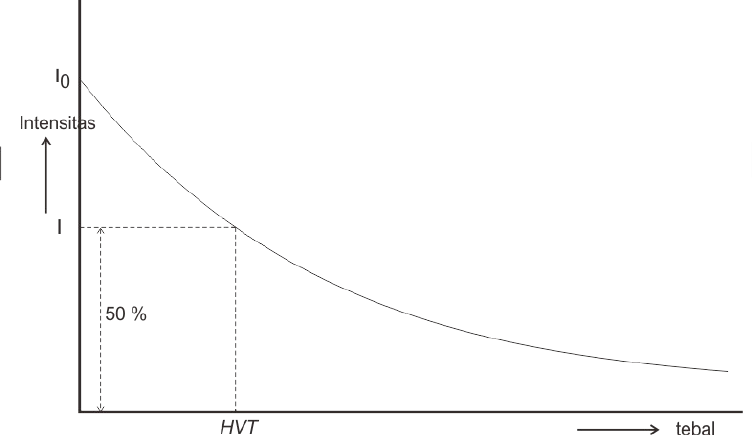
\includegraphics{kurva1}
	\caption{Kurva Intensitas Radiasi vs Tebal Bahan}
	\label{contohgambar}
\end{figure}

\subsubsection{Tabel}
Judul tabel diletakkan di atas dengan rata tengah (center). Tabel \ref{contohtabel} adalah contoh tabel. Font dan penampakan tabel disesuaikan agar tabel tampak bagus dan mudah dibaca. Spasi single. Tabel harus dirujuk di dalam narasi dengan perintah yang sama seperti bagian \ref{gambar}. Makna tabel, baik keterangan maupun nilainya harus dijelaskan. Disarankan letak tabel berada di bagian paling atas atau paling bawah halaman atau berada di akhir (sub) bab. Lakukan sitasi ketika sebuah tabel diambil dari referensi tertentu. 

\begin{table}[!htb]
	\begin{center}
		\caption[Contoh HVL]{Hasil Percobaan HVL Alumunium vs $^{60}$Co}
		\label{contohtabel}
		\begin{tabular}{ccccc}
			\hline
			Ketebalan (inch) & Cacahan rata-rata & N (cps) & N\textsubscript{0} (cps) & $\ln\left(\frac{N}{N_0}\right)$\\
			\hline
			0.125 & 358.67 & 11.15 & 15.02 & -0.2934\\
			0.08 & 356 & 11.06 & 15.02 & -0.3024\\
			0.02 & 413.33 & 12.98 & 15.02 & -0.1444\\
			\hline
		\end{tabular}
	\end{center}
\end{table}

\subsubsection{Rumus dan Persamaan} \label{rumus}
Rumus dan persamaan dituliskan pada Bab 2. Cara penulisan persamaan menggunakan \code{equation} dan bantuan \code{tabular} seperti ditunjukkan pada Persamaan \ref{contohpersamaan}. Seluruh rumus atau persamaan yang dituliskan harus diacu pada paragraph dan disarankan untuk digunakan pada Bab 3 maupun Bab 4.

\begin{equation}\label{contohpersamaan}
	I=I_0.e^{-\mu.x}
\end{equation}

dengan

\begin{tabular}{lcl} 
	$I_0$ &	= & Intensitas paparan radiasi yang datang (mR/jam)\\
	$I$ &	= & Intensitas paparan radiasi yang diteruskan (mR/jam)\\
	$\mu$ &	= & Koefisienn serap linier bahan pada energi tertentu (mm\textsuperscript{-1})\\
	$x$ &	= & Tebal bahan (mm)\\
\end{tabular}

\subsection{Kesalahan penulisan yang sering terjadi}
Disarankan menggunakan kalimat yang lugas dan jelas. Hindari penggunaan anak kalimat yang berlebihan. Jika terpaksa ada anak kalimat, usahakan hanya satu anak saja. Penggunaan banyak anak kalimat atau bahkan beranak cucu akan membingungkan pembaca dalam menangkap maksud kalimat. Gunakan Bahasa Indonesia dengan baik dan benar.

Gunakan tata bahasa secara benar. Pastikan mana yang benar, di mana atau dimana, ke dua atau kedua, dan lain-lain. 

\section{Hipotesis}
Tuliskan hipotesis/pertanyaan penelitian anda berdasarkan tujuan penelitian yang ingin dicapai.